\chapter{Tools}

This chapter provides a overview of the various tools that are
provided as part of the Ames Stereo Pipeline, and a summary of their
command line options.

%--------------------------------------------------------------------------
%                                ASP DEBUGGING
%--------------------------------------------------------------------------

\section{stereo}
\label{stereo}

The \texttt{stereo} program is the primary workhorse of the Ames
Stereo Pipeline.  It takes a stereo pair of images that overlap and
creates an output point cloud image that can be processed into a 3D
model or DEM using the \texttt{point2mesh} or \texttt{point2dem}
programs, respectively.

\medskip

Usage:\\
\hspace*{2em}\texttt{ISIS 3> stereo [options] \textit{Left\_input\_image Right\_input\_image output\_file\_prefix}}

\medskip

This release of the stereo pipeline has been specifically designed to
process USGS ISIS \texttt{.cub} files. However, the stereo pipeline
does have the capability to process other types of stereo image pairs
(e.g. image files with a CAHVOR camera model from the NASA MER
rovers).  If you would like to experiment with these features, please
contact us for more information.

The \texttt{\textit{output\_file\_prefix}} is prepended to all
output data files.  For example, setting \texttt{\textit{output\_file\_prefix}}
to `\texttt{out}' will yield files with names like \texttt{out-L.tif}
and \texttt{out-PC.tif}.  To keep stereo pipeline results organized
in sub-directories, we recommend using an output prefix like
`\texttt{results-10-12-09/out}' for \texttt{\textit{output\_file\_prefix}}.  The
\texttt{stereo} program will create a directory called
\texttt{results-10-12-09/out} and place files named \texttt{out-L.tif},
\texttt{out-PC.tif}, etc. in that directory.

\begin{longtable}{|l|p{7.5cm}|}
\caption{Command-line options for stereo}
\label{tbl:stereo}
\endfirsthead
\endhead
\endfoot
\endlastfoot
\hline
Option & Description \\ \hline \hline
\texttt{-\/-help|-h} & Display this help information\\ \hline
\texttt{-\/-threads \textit{integer(=0)}} & Set the number threads to use. 0 means use default defined in the program or in the .vwrc file\\ \hline
\texttt{-\/-session-type|-t pinhole|isis|dg} & Select the stereo session type to use for processing. Usually the program can select this automatically for the file extension.\\ \hline
\texttt{-\/-stereo-file|-s \textit{filename(=./stereo.default)}} & Define the stereo.default file to use\\ \hline
\texttt{-\/-left-image-crop-win \textit{xoff yoff xsize ysize}}  & Do stereo in a subregion of the left image [default: use the entire image].\\ \hline
\texttt{-\/-entry-point|-e 1|2|3|4} & Pipeline entry point \\ \hline
\end{longtable}

More information about the stereo.default configuration file can be
found in Appendix \ref{ch:stereodefault} on page
\pageref{ch:stereodefault}.  Similarly, \texttt{stereo} creates a lot
of files, and they are all described in Appendix
\ref{chapter:outputfiles} on page \pageref{chapter:outputfiles}.

\subsection{Entry Points}
\label{entrypoints}

The \texttt{stereo -e \textit{number}} option can be used to restart
a {\tt stereo} job partway through the stereo correlation process.
Restarting can be useful when debugging while iterating on {\tt
stereo.default} settings.

Stage 0 (Preprocessing) normalizes the two images and aligns them
by locating interest points and matching them in both images. The
program is designed to reject outlying interest points.  This stage
writes out the pre-aligned images and the image masks.

Stage 1 (Disparity Map Initialization) performs pyramid correlation and builds a rough disparity map that is used to seed the sub-pixel refinement phase.

Stage 2 (Sub-pixel Refinement) performs sub-pixel correlation that
refines the disparity map.

Stage 3 (Outlier Rejection and Hole Filling) performs filtering of the
disparity map and (optionally) fills in holes using an inpainting
algorithm.  This phase also creates a ``good pixel'' map.

Stage 4 (Triangulation) generates a 3D point cloud from the disparity
map.

\subsection{Decomposition of Stereo}

The \texttt{stereo}
executable is a python script that makes calls to seperate
C++ executables for each entry point.

Stage 0 (Preprocessing) calls \texttt{stereo\_pprc}. Multithreaded.

Stage 1 (Disparity Map Initialization) calls
\texttt{stereo\_corr}. Multithreaded.

Stage 2 (Sub-pixel Refinement) class \texttt{stereo\_rfne}. Multithreaded.

Stage 3 (Outlier Rejection and Hole Filling) calls
\texttt{stereo\_fltr}. Multithreaded.

Stage 4 (Triangulation) calls \texttt{stereo\_tri}. Single-Threaded.

All of the sub-programs have the same interface as
\texttt{stereo}. Users processing a large number of stereo pairs on a
cluster my find it advantageous to call these executables in their own
manner. An example would be to run stages 0-3 in order for each stereo
pair. Then run several sessions of \texttt{stereo\_tri} since it is
single threaded.

\section{disparitydebug}
\label{disparitydebug}

The \texttt{disparitydebug} program produces output images for
debugging disparity images created from \verb#stereo#. The {\tt
stereo} tool produces several different versions of the disparity
map; the most important ending with extensions \verb#*-D.tif# and
\verb#*-F.tif#. (see Appendix \ref{chapter:outputfiles} for more
information.)  These raw disparity map files can be useful for
debugging because they contain raw disparity values as measured by
the correlator; however they cannot be directly visualized or opened
in a conventional image browser.  The \verb#disparitydebug# tool
converts a single disparity map file into two normalized TIFF image
files (\verb#*-H.tif# and \verb#*-V.tif#, containing the horizontal
and vertical, or line and sample, components of disparity, respectively)
that can be viewed using any image display program.

The {\tt disparitydebug} program will also print out the range of
disparity values in a disparity map, that can serve as useful summary
statistics when tuning the search range settings in the
{\tt stereo.default} file.

\begin{longtable}{|l|p{10cm}|}
\caption{Command-line options for disparitydebug}
\label{tbl:disparitydebug}
\endfirsthead
\endhead
\endfoot
\endlastfoot
\hline
Options & Description \\ \hline \hline
\texttt{-\/-help|-h} & Display this help\\ \hline
\texttt{-\/-input-file \textit{filename}} & Explicitly specify the input file \\ \hline
\texttt{-\/-output-prefix|-o \textit{filename}} & Specify the output file prefix \\ \hline
\texttt{-\/-output-filetype|-t \textit{type(=tif)}} & Specify the outfile type \\ \hline
\texttt{-\/-float-pixels} & Save the resulting debug images as 32 bit floating point files (if supported by the selected file type) \\ \hline
\end{longtable}

%--------------------------------------------------------------------------
%                           VISUALIZATION TOOLS
%--------------------------------------------------------------------------

\section{point2dem}
\label{point2dem}

The \texttt{point2dem} program produces a GeoTIFF terrain model or/and
an orthographic image from a point cloud image produced by the {\tt
  stereo} command.

Example:\\
\hspace*{2em}\texttt{point2dem \textit{output-prefix}-PC.tif -o stereo/filename -r moon $\backslash$} \\
\hspace*{4em}\texttt{-\/-nodata-value -10000 -n}

This produces a digital elevation model that has been referenced to
the lunar spheroid of 1737.4~km.  Pixels with no data will be set to a
value of -10000, and the resulting \ac{DEM} will be saved in a simple
cylindrical map projection.  The resulting \ac{DEM} is stored by default as
a one channel, 32-bit floating point GeoTIFF file.

The {\tt -n} option creates an 8-bit, normalized version of the DEM
that can be easily loaded into a standard image viewing application
for debugging.

Another example: \\
\hspace*{2em}\texttt{point2dem \textit{output-prefix}-PC.tif -o stereo/filename -r moon $\backslash$} \\
\hspace*{4em}\texttt{-\/-orthoimage \textit{output-prefix}-L.tif}

This command takes the left input image and orthographically projects
it onto the 3D terrain produced by the Stereo Pipeline.  The resulting
{\tt *-DRG.tif} file will be saved as an 8-bit GeoTIFF image in a
simple cylindrical map projection.

\subsection{Comparing with MOLA data}

When comparing the output of \texttt{point2dem} to laser altimeter
data, like MOLA, it is important to understand the different kinds
of data that are being discussed.  By default, \texttt{point2dem}
returns planetary radius values in meters.  These are often large
numbers that are difficult to deal with.  If you use the \texttt{-r
mars} option, the output terrain model will be in meters of elevation
with reference to the IAU reference spheroid for Mars: 3,396,190~m.
So if a post would have a radius value of 3,396,195 m, in the model
returned with the \texttt{-r mars} option, that pixel would just be 5 m.

You may want to compare the output to MOLA data.  MOLA data is
released in three `flavors,' namely: Topography, Radius, and Areoid.
The MOLA Topography data product that most people use is just the MOLA Radius
product with the MOLA Areoid product subtracted.  Additionally, it is
important to note that all of these data products have a reference
value subtracted from them.  The MOLA reference value is NOT the
IAU reference value, but 3,396,000 m.

So you cannot just compare the output of \texttt{point2dem}
to the MOLA Topography data, since \texttt{point2dem} doesn't know about the Areoid.

In order to compare with the MOLA data, you can do one of two
different things.  You could operate purely in radius space, and
have \texttt{point2dem} create radius values that are directly
comparable to the MOLA Radius data.  You can do this by having
\texttt{point2dem} subtract the MOLA reference value by setting
\texttt{-\/-semi-major-axis 3396000} and \texttt{-\/-semi-minor-axis
3396000}.

To get values that are directly comparable to MOLA Topography data,
you'll need to run \texttt{point2dem} with the \texttt{-\/-semi-major-axis}
and \texttt{-\/-semi-minor-axis} switches with the MOLA reference, to get
something that is comparable with the MOLA Radius values.  Then you'll need
to obtain the MOLA Areoid data and scale it up to the DEM ground scale, and then
subtract that areoid data from the model produced by \texttt{point2dem}.  That
resultant model can then be directly compared to the MOLA Topography data.

\subsection{Post Spacing}

Recall that \texttt{stereo} creates a pointcloud file as its output
that you need to use \texttt{point2dem} on to create a GeoTIFF that
you can use in other tools.  The pointcloud file is the result of
taking the image-to-image matches (which were created from the
kernel sizes you specified, and the subpixel versions of the same,
if used) and projecting them out into space from the cameras, and
arriving at a point in real world coordinates.  Since \texttt{stereo} does
this for every pixel in the input images, the \emph{default} value that
\texttt{point2dem} uses (if you don't specify anything explicitly) is: the
input image scale, because there's an `answer' in the pointcloud
file for each pixel in the original image.

However, as you may suspect, this is probably not the best value to
use, because there really isn't that much `information' in the data.
The true `resolution' of the output model is dependent on a whole
bunch of things (like the kernel sizes you choose to use) but also can
vary from place to place in the image depending on the texture.

The general `rule of thumb' is to produce a terrain model that has a
post spacing of about 3x the input image ground scale.  This is based
on the fact that it is nearly impossible to uniquely identify a single
pixel correspondence between two images, but a 3x3 patch of pixels
provides improved matching reliability.  As you go to numerically
larger post-spacings on output, you're averaging more point data (that
is probably spatially correlated anyway) together.

So you can either use the \texttt{-\/-dem-spacing} argument to
\texttt{point2dem} to do that directly, or feel free to use your
favorite averaging algorithm to reduce the \texttt{point2dem}-created
model down to the scale you want.

If you attempt to derive science results from an ASP-produced terrain model
with the default DEM spacing, expect serious questions from reviewers.


\begin{longtable}{|l|p{10cm}|}
\caption{Command-line options for point2dem}
\label{tbl:point2dem}
\endfirsthead
\endhead
\endfoot
\endlastfoot
\hline
Options & Description \\ \hline \hline
\texttt{-\/-nodata-value \textit{float(=min-z)}} & Explicitly set the default missing pixel value. By default, the minimum z value in the model is used. \\ \hline
\texttt{-\/-use-alpha} & Create images that have an alpha channel \\ \hline
\texttt{-\/-normalized|-n} & Also write a normalized version of the \ac{DEM} (for debugging) \\ \hline
\texttt{-\/-orthoimage \textit{texture-file}} & Write an orthoimage based on the texture file given as an argument to this command line option \\ \hline
\texttt{-\/-errorimage} & Write an additional image whose values represent the triangulation error in meters \\ \hline
\texttt{-\/-fsaa  \textit{float(=3)}} & Oversampling amount to perform antialiasing. \\ \hline
\texttt{-\/-output-prefix|-o \textit{output-prefix}} & Specify the output prefix \\ \hline
\texttt{-\/-output-filetype|-t \textit{type(=tif)}} & Specify the output file type \\ \hline
\hline
\texttt{-\/-x-offset \textit{float(=0)}} & Add a horizontal offset to the \ac{DEM} \\ \hline
\texttt{-\/-y-offset \textit{float(=0)}} & Add a horizontal offset to the \ac{DEM} \\ \hline
\texttt{-\/-z-offset \textit{float(=0)}} & Add a vertical offset to the \ac{DEM} \\ \hline
\texttt{-\/-rotation-order \textit{order(=xyz)}} & Set the order of an euler angle rotation applied to the 3D points prior to \ac{DEM} rasterization \\ \hline
\texttt{-\/-phi-rotation \textit{float(=0)}} & Set a rotation angle phi \\ \hline
\texttt{-\/-omega-rotation \textit{float(=0)}} & Set a rotation angle omega \\ \hline
\texttt{-\/-kappa-rotation \textit{float(=0)}} & Set a rotation angle kappa \\ \hline
\hline
\texttt{-\/-t\_srs \textit{string}} & Target spatial reference set. This mimicks the GDAL option used on their tools. \\ \hline
\texttt{-\/-reference-spheroid|-r moon|mars} & Set a reference surface to a hard coded value. This will override manually set datum information. \\ \hline
\texttt{-\/-semi-major-axis \textit{float(=0)}} & Set the dimensions of the datum in meters\\ \hline
\texttt{-\/-semi-minor-axis \textit{float(=0)}} & Set the dimensions of the datum in meters\\ \hline
\texttt{-\/-sinusoidal} & Save using a sinusoidal projection \\ \hline
\texttt{-\/-mercator} & Save using a Mercator projection \\ \hline
\texttt{-\/-transverse-mercator} & Save using transverse Mercator projection \\ \hline
\texttt{-\/-orthographic} & Save using an orthographic projection \\ \hline
\texttt{-\/-stereographic} & Save using a stereographic projection \\ \hline
\texttt{-\/-lambert-azimuthal} & Save using a Lambert azimuthal projection \\ \hline
\texttt{-\/-utm \textit{zone}} & Save using a UTM projection with the given zone \\ \hline
\texttt{-\/-proj-lat \textit{float}} & The center of projection latitude (if applicable) \\ \hline
\texttt{-\/-proj-lon \textit{float}} & The center of projection longitude (if applicable) \\ \hline
\texttt{-\/-proj-scale \textit{float}} & The projection scale (if applicable) \\ \hline
\texttt{-\/-dem-spacing|-s \textit{float(=0)}} & Set the \ac{DEM} post size (if this value is 0, the post spacing size is computed for you) \\ \hline
\texttt{-\/-threads \textit{int(=0)}} & Select the number of processors (threads) to use.\\ \hline
\texttt{-\/-no-bigtiff} & Tell GDAL to not create bigtiffs.\\ \hline
\texttt{-\/-tif-compress None|LZW|Deflate|Packbits} & TIFF Compression method.\\ \hline
\texttt{-\/-cache-dir \textit{directory(=/tmp)}} & Folder for temporary files. Normally this need not be changed.\\ \hline
\hline
\texttt{-\/-help|-h} & Display this table \\ \hline
\end{longtable}

\section{point2mesh}
\label{point2mesh}

Produces a mesh surface that can be visualized in {\tt osgviewer},
which is a standard 3D viewing application that is part of the open
source OpenSceneGraph package.  \footnote{The full OpenSceneGraph package
is not bundled with the Stereo Pipeline, but the \texttt{osgviewer} program
is.  You can download and install this package separately from
\url{http://www.openscenegraph.org/}.}

Unlike \acp{DEM}, The 3D mesh is not meant to be used as a finished
scientific product.  Rather, it can be used for fast visualization
to create a 3D view of the generated terrain.

The \texttt{point2mesh} program requires a point cloud file and an
optional texture file (\texttt{\textit{output-prefix}-PC.tif} and
normally \texttt{\textit{output-prefix}-L.tif}). When a texture
file is not provided, a 1D texture is applied in the local Z direction
that produces a rough rendition of a contour map.  In either case,
\texttt{point2mesh} will produce a \texttt{\textit{output-prefix}.ive}
file that contains the 3D model in OpenSceneGraph format.

Two options for \texttt{osgviewer} bear pointing out: the \texttt{-l}
flag indicates that synthetic lighting should be activated for the
model, which can make it easier to see fine detail in the model by
providing some real-time, interactive hillshading.  The \verb#-s#
flag sets the sub-sampling rate, and dictates the degree to which
the 3D model should be simplified.  For 3D reconstructions, this
can be essential for producing a model that can fit in memory.  The
default value is 10, meaning every 10th point is used in the X and
Y directions. In other words that mean only $1/10^2$ of the points
are being used to create the model. Adjust this sampling rate
according to how much detail is desired, but remember that large
models will impact the frame rate of the 3D viewer and affect
performance.

Example:\\
\hspace*{2em}\texttt{point2mesh -l -s 2 \textit{output-prefix}-PC.tif \textit{output-prefix}-L.tif}

To view the resulting \texttt{\textit{output-prefix}.ive} file use
\texttt{osgviewer}.

\hspace*{2em}Fullscreen:\\
\hspace*{2em}\texttt{> osgviewer \textit{output-prefix}.ive}

\hspace*{2em}or Windowed:\\
\hspace*{2em}\texttt{> osgviewer \textit{output-prefix}.ive -\/-window 50 50 1000 1000}

Inside \texttt{osgviewer}, the keys L, T, and W can be used to toggle on
and off lighting, texture, and wireframe modes.  The left, middle, and
right mouse buttons control rotation, panning, and zooming of the
model.

\begin{longtable}{|l|p{10cm}|}
\caption{Command-line options for point2mesh}
\label{tbl:point2mesh}
\endfirsthead
\endhead
\endfoot
\endlastfoot
\hline
Options & Description \\ \hline \hline
\texttt{-\/-help|-h} & Display this help \\ \hline
\texttt{-\/-simplify-mesh \textit{float}} & Run OSG Simplifier on mesh, 1.0 = 100\% \\ \hline
\texttt{-\/-smooth-mesh} & Run OSG Smoother on mesh \\ \hline
\texttt{-\/-use-delaunay} & Uses the delaunay triangulator to create a surface from the point cloud. This is not recommended for point clouds with noise issues. \\ \hline
\texttt{-\/-step|-s \textit{integer(=10)}} & Sampling step size for mesher. \\ \hline
\texttt{-\/-input-file \textit{pointcloud-file}} & Explicitly specify the input file \\ \hline
\texttt{-\/-texture-file \textit{texture-file}} & Explicitly specify the texture file \\ \hline
\texttt{-\/-output-prefix|-o \textit{output-prefix}} & Specify the output prefix \\ \hline
\texttt{-\/-output-filetype|-t \textit{type(=ive)}} & Specify the output file type \\ \hline
\texttt{-\/-enable-lighting|-l} & Enables shades and light on the mesh \\ \hline
\texttt{-\/-center} & Center the model around the origin. Use this option if you are experiencing numerical precision issues. \\ \hline
\texttt{-\/-rotation-order \textit{order(=xyz)}} & Set the order of an euler angle rotation applied to the 3D points prior to DEM rasterization \\ \hline
\texttt{-\/-phi-rotation \textit{float(=0)}} & Set a rotation angle phi \\ \hline
\texttt{-\/-omega-rotation \textit{float(=0)}} & Set a rotation angle omega \\ \hline
\texttt{-\/-kappa-rotation \textit{float(=0)}} & Set a rotation angle kappa \\ \hline
\end{longtable}

%% \section{orthoproject}
%% \label{orthoproject}

%% Map projects imagery on to point clouds.
%% Note: This process is not multi-threaded because it uses ISIS which is not thread safe.
%% Example:
%% \begin{verbatim}
%% orthoproject -t isis filename-DEM.tif filename.cub filename.isis_adjust \\
%%         filename-DRG.tif --nodata -10000 --ppd 256
%% \end{verbatim}

%% \begin{longtable}{|l|p{10cm}|}
%% \caption{Command-line options for orthoproject}
%% \label{tbl:orthoproject}
%% \endfirsthead
%% \endhead
%% \endfoot
%% \endlastfoot
%% \hline
%% Options & Description \\ \hline \hline
%% \verb#--help# & Display this table \\ \hline
%% \verb#--mpp arg# & Specify the output resolution of the orthoimage in meters per pixel \\ \hline
%% \verb#--ppd arg# & Specify the output resolution of the orthoimage in pixels per degree \\ \hline
%% \verb#--nodata-value arg# & Specify the pixel used in this DEM to denote missing data \\ \hline
%% \verb#-m# & Match the georeferencing parameters and dimensions of the input DEM \\ \hline
%% \verb#--min arg# & Explicitly specify the range of the normalization (for ISIS images only) \\ \hline
%% \verb#--max arg# & Explicitly specify the range of the normalization (for ISIS images only) \\ \hline
%% \verb#--cache arg# & Cache size, in megabytes \\ \hline
%% \verb#-t arg (=pinhole)# & Select the stereo session type to use for processing. [default: pinhole] \\ \hline
%% \verb#--mark-no-processed-data# & If to set no-data pixels in the DEM which project onto the camera to black. [default: false]
%%                                   This option is used used only for creating images suitable for albedo generation. \\ \hline

%% \verb#-d arg (=29)# & Set the debugging output level. (0-50+) \\ \hline
%% \end{longtable}

\clearpage

\section{orbitviz}
\label{orbitviz}

Produces a Google Earth \ac{KML} file useful for visualizing camera
position. The input for this tool is one or more \texttt{*.cub} files.

\begin{figure}[!b]
  \begin{center}
  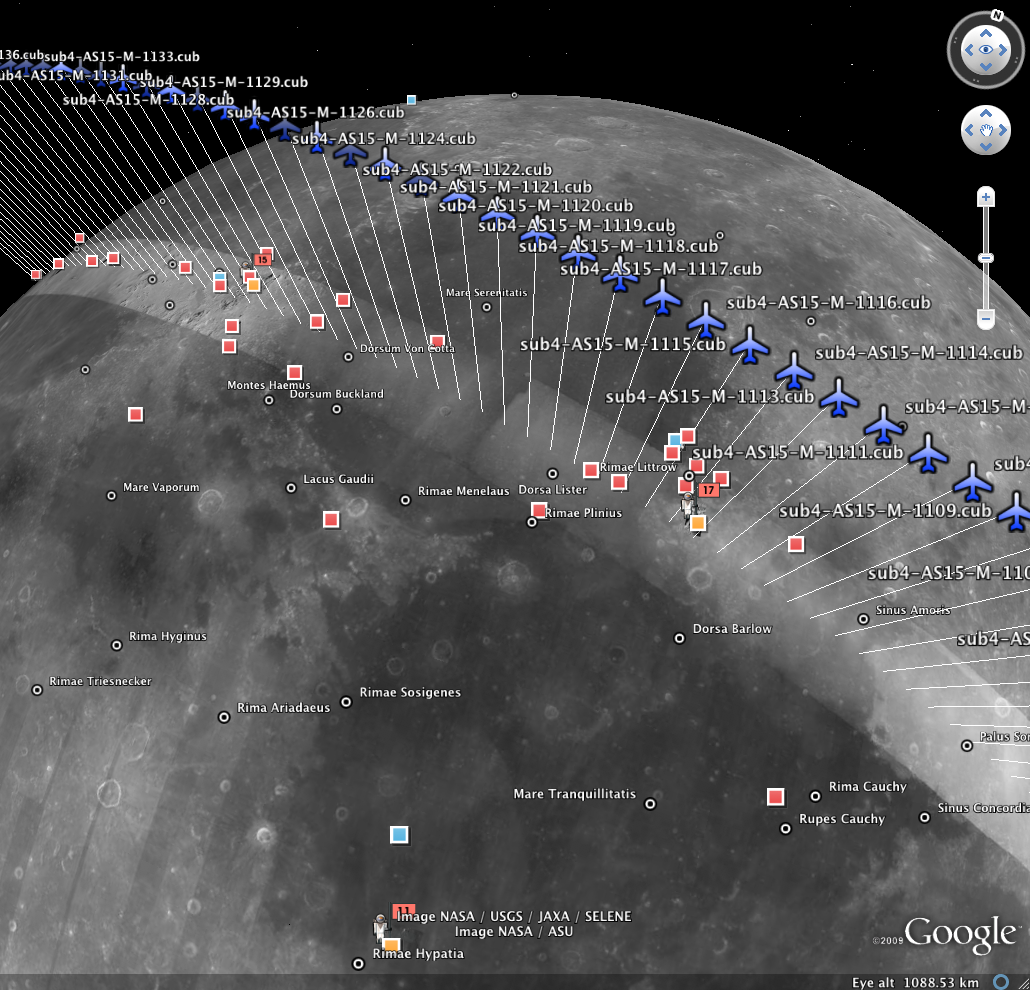
\includegraphics[width=6in]{images/orbitviz_ge_result.png}
  \end{center}
  \caption{ Example of a \ac{KML} visualization produced with {\tt
      orbitviz} depicting camera locations for the Apollo 15 Metric
    Camera during orbit 33 of the Apollo command module.}
  \label{fig:orbitviz_example}
\end{figure}

\begin{longtable}{|l|p{10cm}|}
\caption{Command-line options for orbitviz}
\label{tbl:orbitviz}
\endfirsthead
\endhead
\endfoot
\endlastfoot
\hline
Options & Description \\ \hline \hline
\texttt{-\/-help|-h} & Display this help \\ \hline
\texttt{-\/-output|-o \textit{filename(=orbit.kml)}} & Specifies the output file name \\ \hline
\texttt{-\/-scale|-s \textit{float(=1)}} & Scale the size of the coordinate axes by this amount. Ex: To scale axis sizes up to earth size, use 3.66 \\ \hline
\texttt{-\/-use\_path\_to\_dae\_model|-u \textit{fullpath}} & Use this dae model to represent camera location. \emph{Google Sketch up can create these.} \\ \hline
\end{longtable}

\clearpage

\section{cam2map4stereo.py}
\label{cam2map4stereo}

This program takes similar arguments as the ISIS3 \texttt{cam2map} program,
but takes two input images.  With no arguments, the program determines
the minimum overlap of the two images, and the worst common resolution,
and then map-projects the two images to this identical area and resolution.

The detailed reasons for doing this, and a manual step-by-step walkthrough of
what \texttt{cam2map4stereo.py} does is provided in the disucssion on aligning images on page \pageref{sec:AligningImages}.

The \texttt{cam2map4stereo.py} is also useful for selecting a subsection and/or reduced resolution portion of the full image.  You can inspect a raw camera geometry image in qview after you have run \texttt{spiceinit} on it, select the latitude and longitude ranges, and then use \texttt{cam2map4stereo.py}'s \texttt{-\/-lat}, \texttt{-\/-lon}, and optionally \texttt{-\/-resolution} options to pick out just the part you want.

Use the \texttt{-\/-dry-run} option the first few times to get an idea of what \texttt{cam2map4stereo.py} does for you.

\begin{longtable}{|l|p{10cm}|}
\caption{Command-line options for cam2map4stereo.py}
\label{tbl:bundlevis}
\endfirsthead
\endhead
\endfoot
\endlastfoot
\hline
Options & Description \\ \hline \hline
\texttt{-\/-help|-h} & Display this help \\ \hline
\texttt{-\/-manual} & Read the manual. \\ \hline
\texttt{-\/-map=\textit{MAP}|-m \textit{MAP}} & The mapfile to use for \texttt{cam2map}. \\ \hline
\texttt{-\/-pixres=\textit{PIXRES}|-p \textit{PIXRES}} & The pixel resolution mode to use for \texttt{cam2map}. \\ \hline
\texttt{-\/-resolution=\textit{RESOLUTION}|-r \textit{RESOLUTION}} & Resolution of the final map for \texttt{cam2map}. \\ \hline
\texttt{-\/-interp=\textit{INTERP}|-i \textit{INTERP}} & Pixel interpolation scheme for \texttt{cam2map}. \\ \hline
\texttt{-\/-lat=\textit{LAT}|-a \textit{LAT}} & Latitude range for \texttt{cam2map}, where \texttt{LAT} is of the form \textit{min:max}.  So to specify a latitude range between -5 and 10 degrees, it would look like \texttt{-\/-lat=-5:10}. \\ \hline
\texttt{-\/-lon=\textit{LON}|-o \textit{LON}} & Longitude range for \texttt{cam2map}, where \texttt{LON} is of the form \textit{min:max}.  So to specify a longitude range between 45 and 47 degrees, it would look like \texttt{-\/-lon=40:47}. \\ \hline
\texttt{-\/-dry-run|-n} & Make calculations, and print the \texttt{cam2map} command that would be executed, but don't actually run it.\\ \hline
\texttt{-\/-suffix|-s} & Suffix that gets inserted in the output file names, defaults to `map'.\\ \hline
\end{longtable}

\clearpage

\section{dem\_adjust}
\label{demadjust}

Takes as input a DEM of Earth whose height values are relative to the
WGS84 ellipsoid, and adjusts those values to be relative to the
geoid. The program can also apply the reverse of this adjustment.

Two geoids are supported: EGM96
(\url{http://earth-info.nga.mil/GandG/wgs84/gravitymod/egm96/egm96.html})
and NAVD88 (\url{http://www.ngs.noaa.gov/GEOID/GEOID09/}).

It is important to note that the NAVD88 geoid is strictly speaking in
reference to the NAD83 ellipsoid rather than to WGS84 as we assume
here. These two ellipsoids have minor differences in parameters.

\begin{longtable}{|l|p{10cm}|}
\caption{Command-line options for dem\_adjust}
\label{tbl:demadjust}
\endfirsthead
\endhead
\endfoot
\endlastfoot
\hline
Options & Description \\ \hline \hline
\texttt{-\/-help|-h} & Display this help \\ \hline
\texttt{-\/-nodata-value \textit{=-32767}} & The value of no-data pixels, unless specified in the DEM \\ \hline
\texttt{-\/-geoid \textit{=EGM96}} & The geoid to use [EGM96, NAVD88] \\ \hline
\texttt{-\/-output-prefix|-o \textit{filename}} & Specify the output file prefix \\ \hline
\texttt{-\/-double} & Output using double precision (64 bit) instead of float (32 bit)\\ \hline
\texttt{-\/-reverse-adjustment} & Go from DEM relative to the geoid to DEM relative to the ellipsoid\\ \hline
\end{longtable}


%% \section{reconstruct}
%% \label{reconstruct}

%% Tool under development

%% \section{results}
%% \label{results}

%% Tool under development

%% \section{rmax\_adjust}
%% \label{ramx_adjust}

%% Bundle Adjustment tool specifically for the Yamaha RMAX unmanned
%% aerial vehicle.
